\apendice{Documentación de usuario}
\section{Introducción}
En este apartado se van a detallar los pasos necesarios para ejecutar la aplicación desde el punto de vista del usuario.
\section{Requisitos de usuarios}
Los requisitos mínimos para poder hacer uso de la aplicación son:
\begin{itemize}
	\item Tener instalado \emph{Python 3}
	\item Tener instalado las librerías correspondientes (\emph{Scholarly, Bibtexparser, Selenium, PIL}).En el anexo \ref{instalar} se especifica como se pueden obtener estas librerías.
	\item Disponer de conexión a Internet.
	\item Disponer de acceso a los recursos científicos del \emph{FECYT}, para ello valdría acceso a la red de la universidad o bien una VPN a esta red si se pretende trabajar desde casa.
	\item Cuenta registrada en la aplicación web ACADEMIA. para ello basta con acceder al enlace \cite{registro} y cumplimentar los datos de registro.
\end{itemize}
\section{Instalación}
Para la ejecución de la aplicación no es necesario una instalación tradicional del proyecto, simplemente es necesario clonar o descargar el repositorio desde \emph{GitHub} y ejecutarlo como se ha indicado en el Anexo \ref{ejecutar}
\section{Manual del usuario}
A continuación, vamos a explicar los pasos a seguir por parte de un usuario cualquiera para un correcto uso de la aplicación.

\subsection{Introducción de datos}
Nada más ejecutar la aplicación se nos presentará la siguiente interfaz:
\begin{figure}[H]
	\centering
	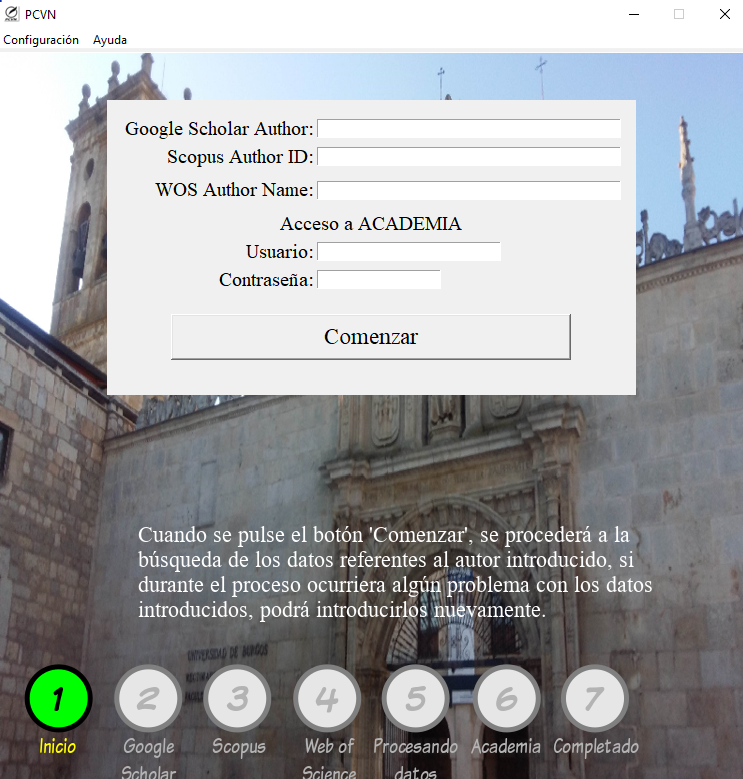
\includegraphics[width=0.8\textwidth]{GUI1}
	\caption{Imagen de ejemplo de uso.}
\end{figure}
en la que como vemos existen una serie de recuadros donde se ha de introducir el identificador para cada una de las páginas (Nombre, ID, Nombre, Usuario y contraseña). En el cuadro de texto de la parte inferior observamos que se nos indica que es lo que va a suceder a continuación. Esto sería un uso completo de la aplicación, es decir se buscan las publicaciones de un autor, se procesan y con las credenciales introducidas por el usuario se suben a su cuenta de ACADEMIA. Sin embargo, con el menú desplegable que podemos ver en la parte superior de la imagen podemos cambiarlo, este menú nos permite:
\begin{itemize}
	\item Configurar el número máximo de publicaciones que queremos extraer.
	
	\begin{figure}[H]
	\centering
	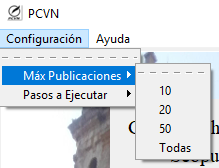
\includegraphics[width=0.5\textwidth]{GUI_menu1}
	\caption{Imagen configuración de publicaciones.}
	\end{figure}
	
	\item Configurar que procesos queremos llevar acabo. La opción por defecto es el uso completo de la aplicación, si bien podemos elegir cual de los procesos se quiere llevar a cabo. Según sea nuestra elección se nos cambiará a una u otra ventana y se adaptaran los textos informativos para informarnos fielmente de lo que va a ocurrir.
	
	\begin{figure}[H]
	\centering
	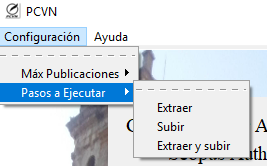
\includegraphics[width=0.5\textwidth]{GUI_menu2}
	\caption{Imagen configuración de procesos a ejecutar.}
	\end{figure}
	
	\item Ayuda, que nos abrirá un documento \emph{pdf} que ofrece ayuda sobre el correcto uso de la aplicación.
\end{itemize}

Vamos a seguir la ejecución completa del proceso pues engloba el resto de opciones a elegir.\\ Una vez introducidos los datos pulsamos sobre el botón \emph{Comenzar}. Entonces se producirá un cambio en la interfaz que indica que se está procediendo a la extracción de datos.
En este punto pueden ocurrir 2 cosas:

\begin{itemize}
	\item Todo vaya según lo previsto, entonces se mostrará una interfaz como la siguiente:
	\begin{figure}[H]
	\centering
	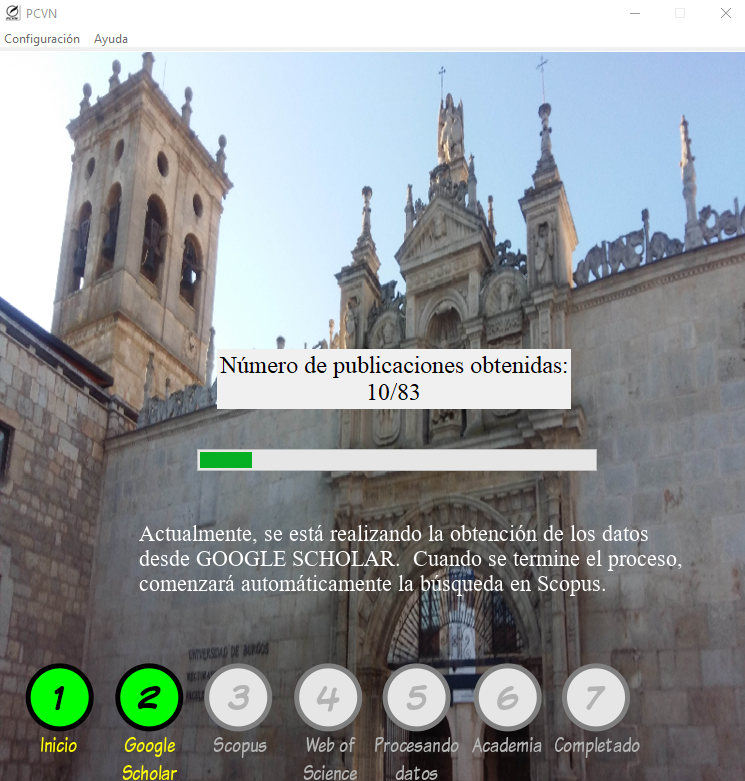
\includegraphics[width=0.8\textwidth]{GUI2}
	\caption{Imagen de extracción de información de \emph{Google Search}.}
	\end{figure}
	Una vez completada la barra saltará al siguiente proceso.
	\item Exista algún problema con la ejecución, por ejemplo, no se disponga de conexión a Internet o los datos introducidos para el autor no generan ningún resultado. Entonces se mostrará la siguiente interfaz:
		\begin{figure}[H]
	\centering
	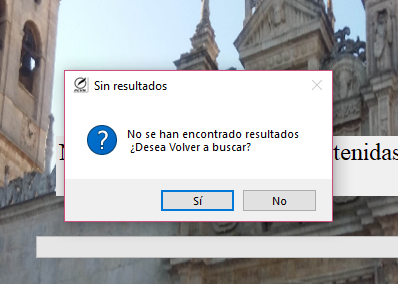
\includegraphics[width=0.6\textwidth]{GUI_error_gs}
	\caption{Imagen de error en el proceso de búsqueda de \emph{Google Search}.}
	\end{figure}
	Dependiendo del error que se haya producido (Sin conexión, Sin resultados, etc.) se mostrará un mensaje u otro en la ventana emergente.Ahora volvemos a tener dos opciones:
	\begin{itemize}
		\item Volver a introducir los datos referentes al autor, pero esta vez únicamente para \emph{Google Search}. como vemos en la siguiente imagen.
		\begin{figure}[H]
	\centering
	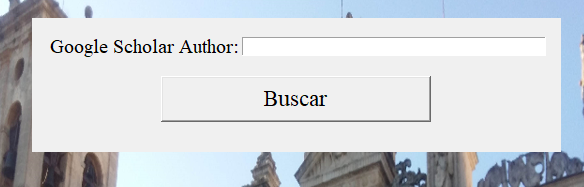
\includegraphics[width=0.8\textwidth]{gui_scholar_resch}
	\caption{Imagen de vuelta a buscar en \emph{Google Search}}
	\end{figure}
		\item Finalizar aquí la ejecución de la aplicación.
	\end{itemize}
\end{itemize}

Una vez finalizado el proceso anterior correctamente se procederá automáticamente a realizar la extracción de los datos de \emph{Scopus} con un nuevo cambio en la interfaz y donde nos puede ocurrir algo similar a lo acontecido en el paso anterior:
\begin{itemize}
	\item Todo vaya según lo previsto con lo que se procederá a la extracción de los datos.
	
	\begin{figure}[H]
	\centering
	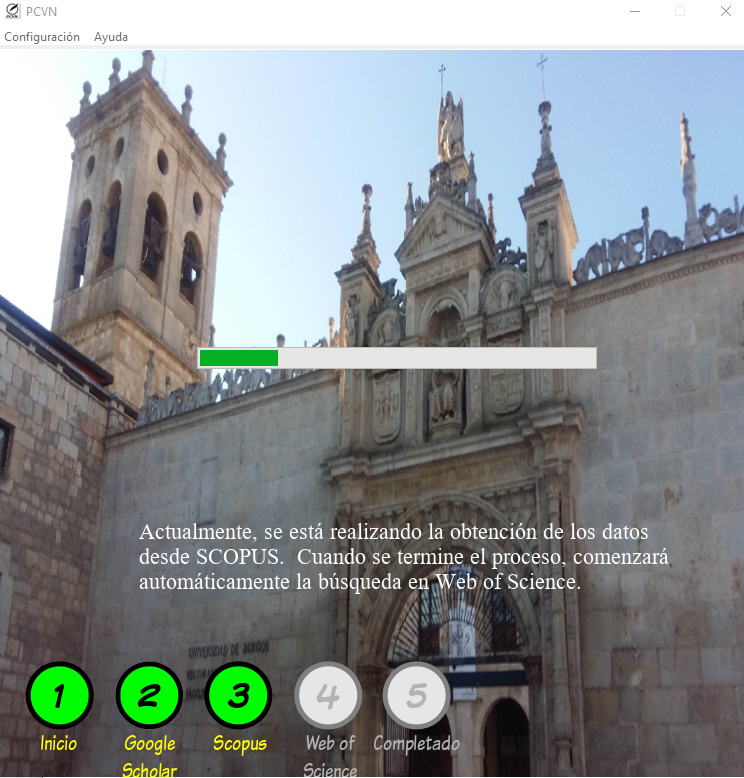
\includegraphics[width=0.8\textwidth]{GUI_scopus}
	\caption{Imagen de búsqueda en \emph{Scopus}}
	\end{figure}
	
	\item Que se detecte algún problema con los datos o la conexión, lo que termine en una nueva introducción de datos.
	
	\begin{figure}[H]
	\centering
	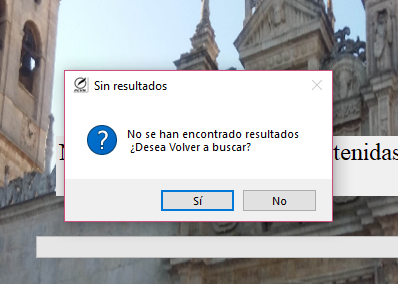
\includegraphics[width=0.8\textwidth]{GUI_error_gs}
	\caption{Imagen de error en el proceso de búsqueda de \emph{Scopus}.}
	\end{figure}
	
	Aquí se nos vuelven a presentar una serie de opciones:
	\begin{itemize}
		\item Volver a introducir los datos referentes al autor 
			
		\begin{figure}[H]
		\centering
		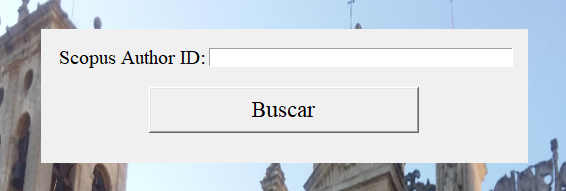
\includegraphics[width=0.8\textwidth]{gui_scopus_rsch}
		\caption{Imagen de volver a buscar en \emph{Scopus}.}
		\end{figure}
	
		\item Finalizar aquí la ejecución de la aplicación.
		\item En el caso de que se haya tratado de otro tipo de error (de conexión , error interno ,etc.) se podrá reintentar el proceso con los mimos datos.
	\end{itemize}
\end{itemize}
Una vez finalizado este proceso correctamente automáticamente habrá un cambio en la interfaz que indica que se ha procedido con el siguiente proceso de extracción exactamente igual que en los pasos anteriores, donde nos puede ocurrir:
\begin{itemize}
	\item Todo vaya según lo previsto con lo que se procederá a la extracción de los datos.
				
		\begin{figure}[H]
		\centering
		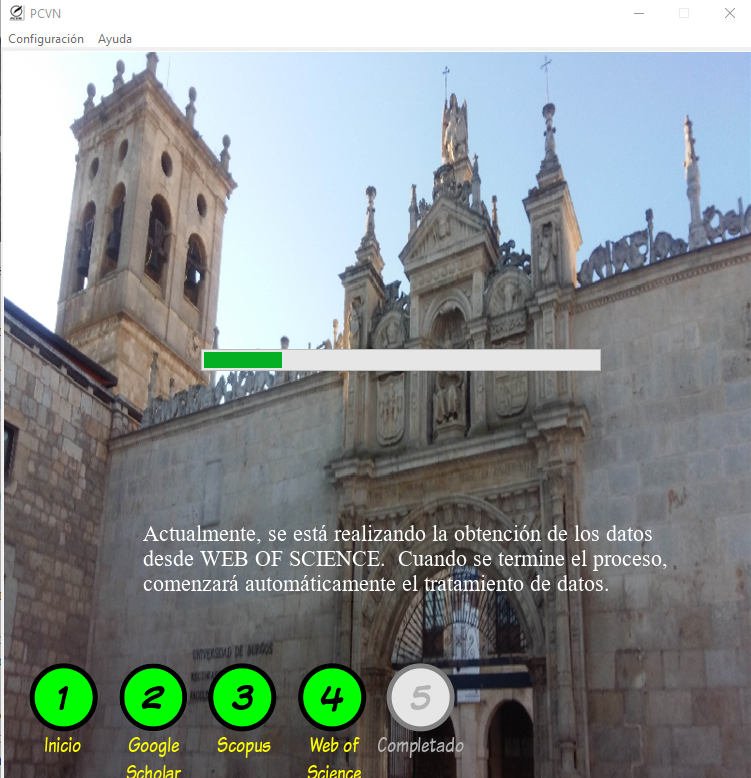
\includegraphics[width=0.8\textwidth]{GUI_wos}
		\caption{Imagen de extracción de información de\emph{Web of Science}.}
		\end{figure}
	
	\item Que se detecte algún problema con los datos o la conexión, lo que termine en una nueva introducción de datos.
		
	\begin{figure}[H]
	\centering
	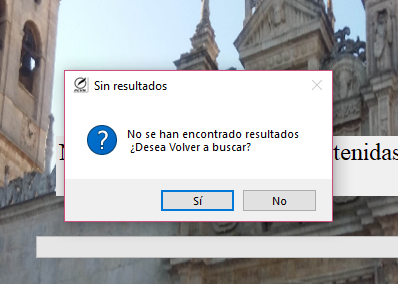
\includegraphics[width=0.8\textwidth]{GUI_error_gs}
	\caption{Imagen de error en el proceso de búsqueda de \emph{Web of Science}.}
	\end{figure}
	Aquí se nos vuelven a presentar una serie de opciones:
	\begin{itemize}
		\item Volver a introducir los datos referentes al autor 
			
		\begin{figure}[H]
		\centering
		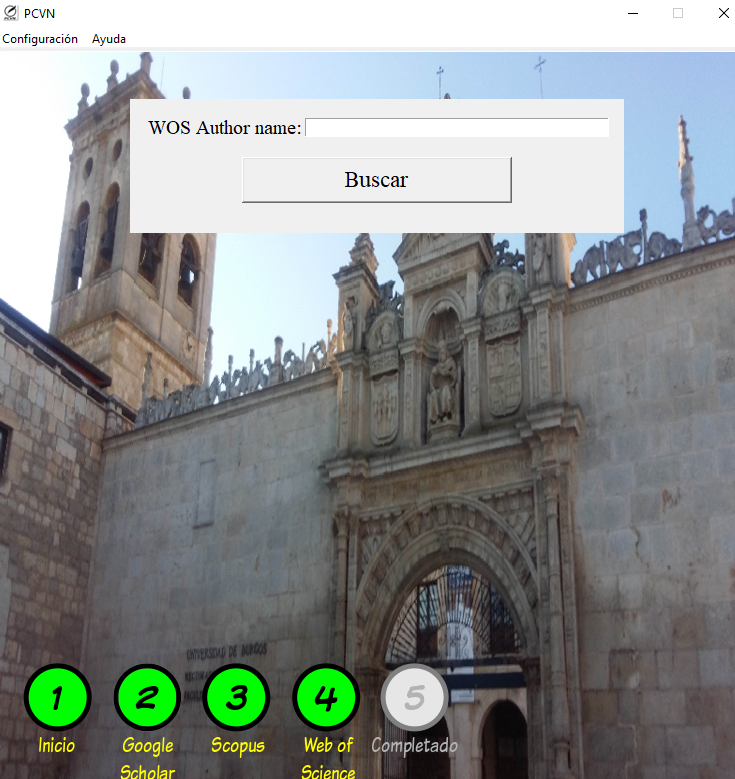
\includegraphics[width=0.8\textwidth]{gui_wos_rsch}
		\caption{Imagen de volver a buscar en \emph{Web of Science}.}
		\end{figure}
	
		\item Finalizar aquí la ejecución de la aplicación.
		\item En el caso de que se haya tratado de otro tipo de error (de conexión , error interno ,etc.) se podrá reintentar el proceso con los mimos datos.
	\end{itemize}
\end{itemize}

Cuando esta última extracción haya concluido se procederá al tratamiento de datos,	en donde simplemente habrá que esperar a que termine el proceso. Para ayudar en la visualización del progreso como en el resto de las partes de la interfaz se dispone de una barra de progresos que indica la carga de trabajo realizada.

		\begin{figure}[H]
		\centering
		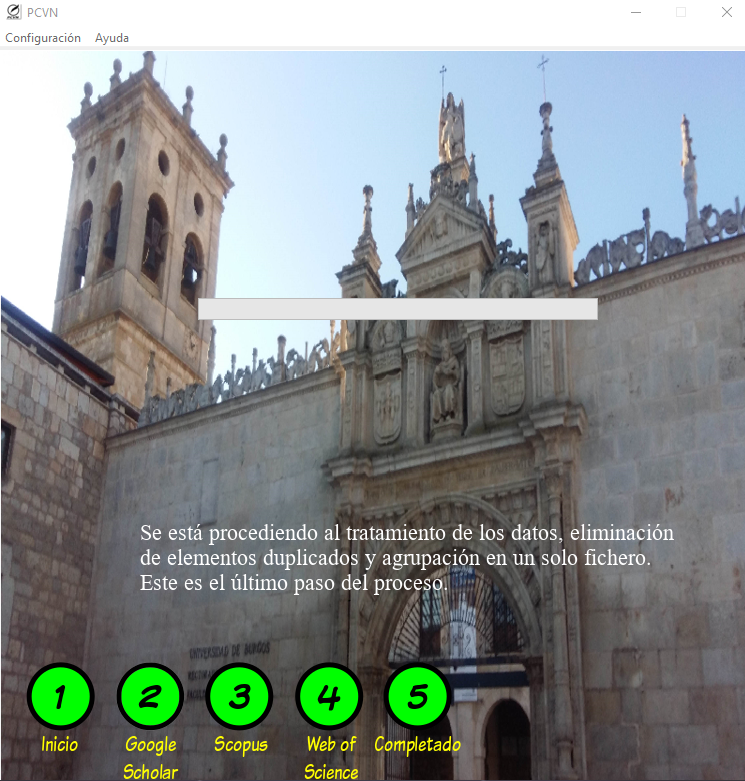
\includegraphics[width=0.8\textwidth]{GUI_procesado}
		\caption{Imagen del procesado de datos.}
		\end{figure}
		
En el caso de que se haya decidido realizar únicamente el proceso de extracción de los datos, este habría sido el último paso del proceso y se nos abriría una ventana que nos permitiría ver las publicaciones que hayan sido extraídas o bien finalizar completamente la aplicación como se ve en la siguiente imagen:

		\begin{figure}[H]
		\centering
		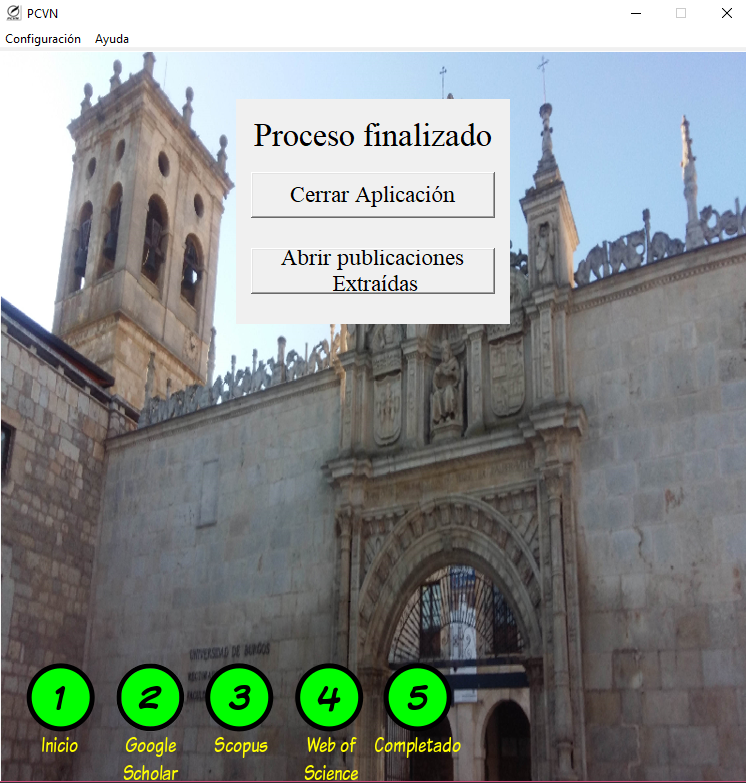
\includegraphics[width=0.8\textwidth]{GUI_fin_extr}
		\caption{Imagen final del proceso de extracción datos.}
		\end{figure}
		
En el caso de que se haya decido saltar el proceso de extracción de datos y se haya decidido realizar solo la subida de los datos (aportando el fichero con las publicaciones a subir), se mostrará una nueva interfaz donde se deberá introducir el nombre del autor, el usuario (DNI,NIE) y la contraseña para poder acceder a la plataforma y que comience el proceso de subida de los datos previamente extraídos. Como se puede ver en la siguiente imagen:
			
		\begin{figure}[H]
		\centering
		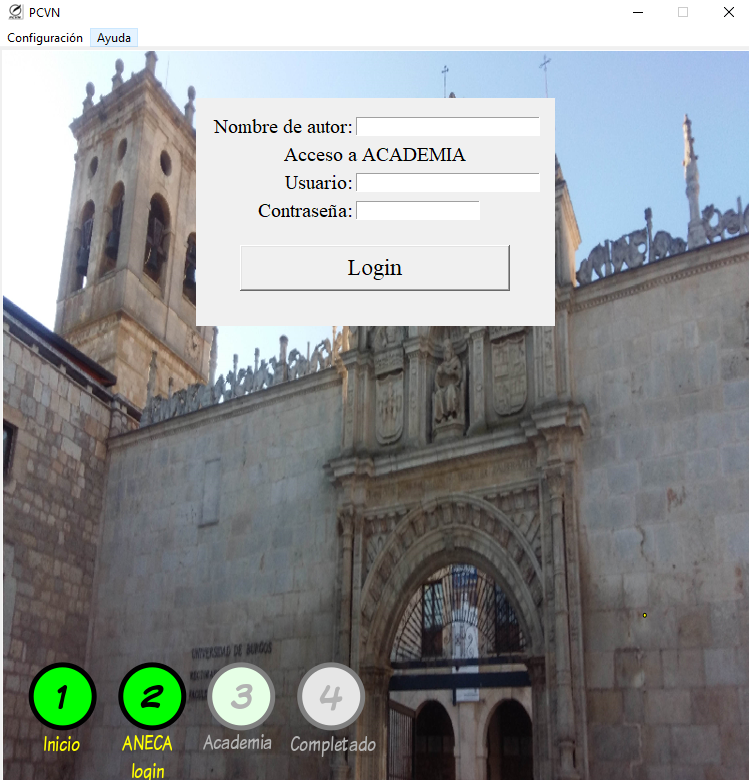
\includegraphics[width=0.8\textwidth]{GUI_login}
		\caption{Imagen de inicio de sesión.}
		\end{figure}
	

De nuevo pueden ocurrir dos cosas:
\begin{itemize}
	\item El usuario y contraseña sean correctos, con lo que se procederá con normalidad.
	\item El usuario y contraseña no sean correctos, por lo volverán a ser solicitados.
\end{itemize}
En el caso de que se haya decidido realizar el proceso completo (extracción y subida) no será necesaria la identificación pues ya se ha realizado al inicio del proceso y seguiríamos directamente con el proceso de subida de los datos. \\

Una vez debidamente identificado en la aplicación ACADEMIA se comenzará la subida de datos. De nuevo tendremos una barra de progreso que nos indica el progreso respecto del total y un cuadro de texto que nos indica que tipo de publicación se está subiendo y el número respecto el total.

		\begin{figure}[H]
		\centering
		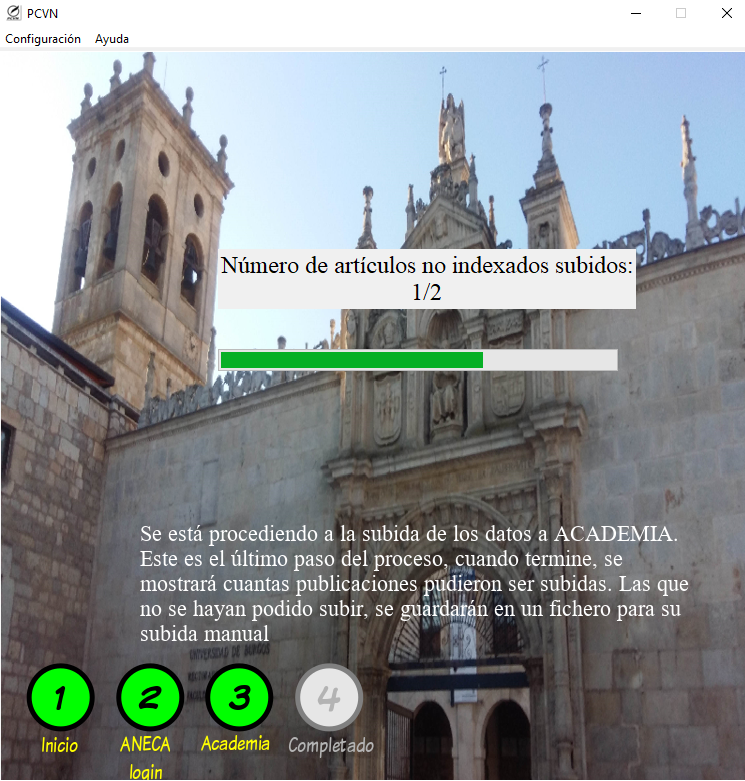
\includegraphics[width=0.8\textwidth]{GUI_subida}
		\caption{Imagen del proceso de subida.}
		\end{figure}


Para finalizar se nos muestra una pantalla final con información del número total de publicaciones y el número de publicaciones que por error de formato no han podido ser subidas. Estas publicaciones no se perderán si no que han sido guardadas en un fichero específico para una posterior revisión por parte del usuario.

		\begin{figure}[H]
		\centering
		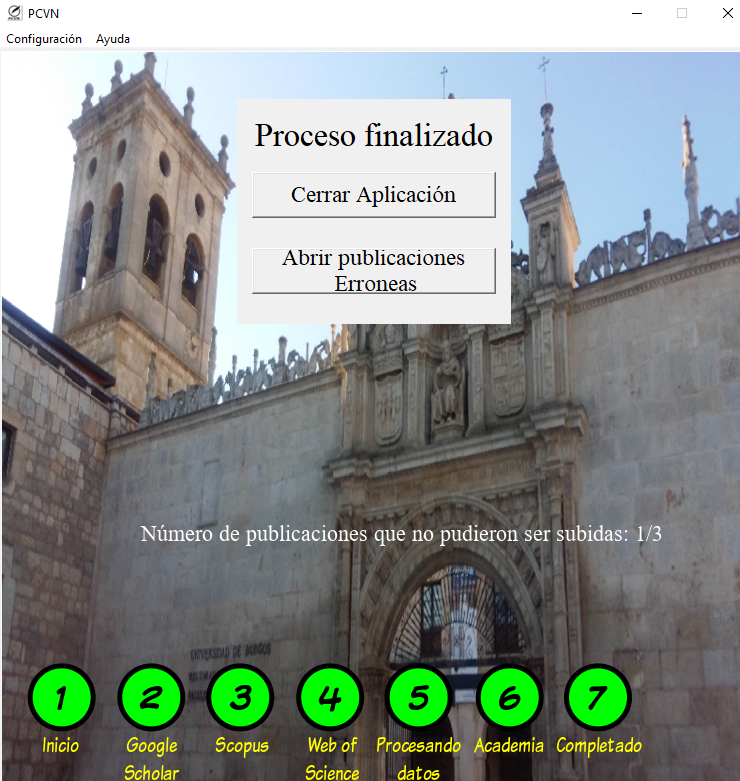
\includegraphics[width=0.8\textwidth]{GUI_completado}
		\caption{Imagen final del proceso de subida.}
		\end{figure}

